\chapter{Introduction}
\label{chap/intro} 

Three dimensional object recognition is a fundamental problem in computer vision. It encompasses detection, identification, classificaiton and pose estimation of 3D objects and time-varying 2D visual data in general, including point clouds, depth maps, volumetric data and videos. 

The topics of 3D object recognition were studied extensively since the early days of computer vision research. 
% Pioneer articulated very different framework for representing and recognising 3D objects. 
Pioneers of computer vision have proposed various models for representing and recognising objects from 3D data.
% The number of literature reflected how the early researher treat the topic seriously. 
% Marr 
For instance, Marr and Nishihara \cite{Marr1978} presented the primal sketch, in which an 3D object is represented as a hierarchical set of cylinders positioned in an object-centric frame. 
% Generalised cone by Nevatia 
In addition, Nevatia and Binford \cite{Nevatia1977} proposed the generalised cones framework to describe and recognise 3D objects. Bolles \etal \cite{Bolles1983} studied the pose estimation of 3D objects from depth maps.
% Moving light display 
Concerning object recognition in video data, Johansson \cite{Johansson1973} pioneered video-based action recognition using a moving light display. 
% Nevertheless, practical applications of such early models are limited, due to the restrictions in computational power to process large amount of 3D data and the high cost of collecting sufficient data for training and testing.

Practical applications of these early models were limited: Firstly, the computational power available by then was inadequate to process a large amount of 3D data for sophisicated learning algorithms. Secondly, it was too costly to collect sufficient data for training and testing, without the help of contemporary efficient 3D data capturing devices and technologies. Finally, they did not consider occlusions, viewpoints and pose variations which are the archetypal issues in practical object recognition systems. 
Image-based object recognition, being more efficient and attainable, has gradually gained more attention, as it is more applicable than its 3D counterpart. Much work has been done in solving recognition tasks on 2D images, helped by the advent of appearance-based image descriptors and learning-based classifiers, and these methods are now reaching maturity. 

Nevertheless, research interest in 3D object recognition has been rekindled recently. 
With the advent of affordable data acquistiion technologies, such as depth sensors \cite{Shotton2011}, multi-view stereo systems \cite{Vogiatzis2011} and video cameras in mobile devices, pave the way for the return of 3D object recognition data systems. 
Meanwhile, modern computing hardware, along with the availability of large-scale 3D datasets, make fully-automatic 3D object recognition possible using machine learning techniques.  

This thesis addresses the sub-problems of \emph{classification} and \emph{pose-estimation} for \emph{3D geometric shapes} and \emph{human actions in videos}. 
% Videos and 3D shape data are the most accessible representation of 3D object data.
Videos and 3D shapes are the most applicable and accessible representation of 3D spatial and spatiotemporal objects, which can be obtained from video cameras and affordable modern 3D shape acquisition devices, \eg multi-view stereo \cite{Vogiatzis2011} and Kinect sensor \cite{Shotton2011}. 
% Photometric textures on 3D shape surfaces are not considered because they are more costly and difficult to be captured.  
Recently, large-scale benchmark datasets, \eg Princeton shape benchmark \cite{Shilane2004},  KTH action dataset \cite{Schuldt2004}, TOSCA dataset \cite{Bronstein2011} and Youtube video dataset \cite{Liu2009}, have been made available to public, facilitiating standardised comparison among different approaches. 
On the other side, classification and pose estimation are two essential components in many object recognition systems, such as human-computer interface, computer-aided design, automatic fault detection, video surveillance, computer graphics and entertainment. 
Early approaches of 3D shape recognition are discussed in the literature review by Besl and Jain \cite{Besl1985}. Early techniques of video-based human motion classification were reviewed by C\'edras and Shah \cite{Cedras1995}, Moeslund and Granum \cite{Moeslund2001} and Turaga \etal \cite{Turaga2008}. In addition, literature reviews on early human pose estimation techniques were conducted by Aggarwal and Cai \cite{Aggarwal1999} and Poppe \cite{Poppe2007}.  
% Why classification? Maybe add some more\ldots 
% Why pose estimation? Matbe add some more\ldots

This thesis is organised into two parts.  
The first part is concerned with the classification and pose estimation of 3D shapes. It starts with a performance evaluation of interest point detectors for 3D shape data. It then proposes a new semi-supervised deformable part model which performs simultaneous 3D shape classification and pose estimation. In the second part, three new algorithms for human action classification, 3D body pose estimation and 3D hannd pose estimation from videos and depth image sequences are proposed respectively. Experimental results have demonstrated that state-of-the-art performances can be achieved using different variants of random forest algorithms.  

\section{Challenges}

% problems of 3D shape recognition
Although 3D object classification and pose estimation have been studied for decades, there is still much room for improvement in fully-automatic shape or action recognition systems. 
This thesis studies several long-standing challenges in 3D object classification and pose estimation.  

\subsection{3D shape classification and registration} 

Different 3D shape representations lead to diversified features for classification and registration. Designing an generic 3D shape recognition algorithm is therefore difficult. Many existing methods are restricted to certain data representations and formats, especially for triangular mesh which is a standard for synthetic 3D data, \eg Harris3D \cite{Sipiran2011} and MeshHOG \cite{Zaharescu2009}.     
While 2D image-based interest points are studied extensively \cite{Mikolajczyk2005}, there are few comprehensive performance evaluations for 3D interest points. 
Adressing the above issue, this thesis is mainly concerned with the interest points in volumetric data, which is a common representation of 3D and time-varying data. Voxels can be converted conveniently from other data formats, such as point clouds, meshes and videos, providing extra applicability and usability. 

In addition, categorical pose estimation of 3D shapes is another important area in computer vision.
Standard bag-of-words models for 3D object categorisation do not consider object pose, as they disregard the structural information of objects for better robustness. Traditional 3D registration algorithms, such as iterative closest point (ICP) \cite{Besl1992}, do not model the variations among instances within the same object class. 
Generative part-based models provide a supervised framework to infer scale and translation of an object class \cite{Weber2000, Fergus2007}. However, object rotation is not included in the above models. 
Voting-based methods, \eg Gall and Lempitsky \cite{Gall2009a}, performs 3D shape classification and registration simultaneously using generalised Hough transform. However, they require training data to be registered manually in advance.  
To summarise, pose estimation of 3D shapes remains an largely unresolved issue, especially for category-based and unsupervised pose estimation tasks.  

\subsection{Human action classification}

% Computational bottleneck

Bag-of-words is an established approach for video classification tasks \cite{Schuldt2004, Dollar2005, Riemenschneider2009, Niebles2008, Wong2007}. However, its performance is limited because the codeword histograms utilise only appearance features, in an orderless way. Run-time performance is also a major issue in human action classification. Although real-time action classification is essential for many applications, such as human-computer interfaces and video surveillance, existing methods perform classification only after the whole testing sequence has been processed. 

\subsection{3D human pose estimation} 

% uncontrolled environments
% 1. Background
% 2. Special Hardware, multiple cameras  

Recent 3D human pose estimation algorithms have achieved promising performances in controlled environments, \eg \cite{Rogez2012, Pons-Moll2011, Sigal2012}. On the other side, 3D human pose estimation in unconstrained environments is still an unexplored area.       
Traditional pose estimation algorithms often rely on low-level appearance features, such as silhouette and motion templates \cite{Bissacco2007, Rogez2012, Ionescu2011, Navaratnam2006}. These features are vulnerable to dynamic scenes, cluttered backgrounds and moving viewpoints in unconstrained videos. 
Pose ambiguities and self-occlusions are common issues in both body pose and hand pose estimation. While multi-view techniques handle such problems effectively in controlled settings, they are not applicable to unconstrained, monocular testing videos. Additional prior knowledge about the subject's structure, \eg articulated human body or hand, is required to remove such ambiguities in monocular videos. 

\begin{figure}[ht]
\centering
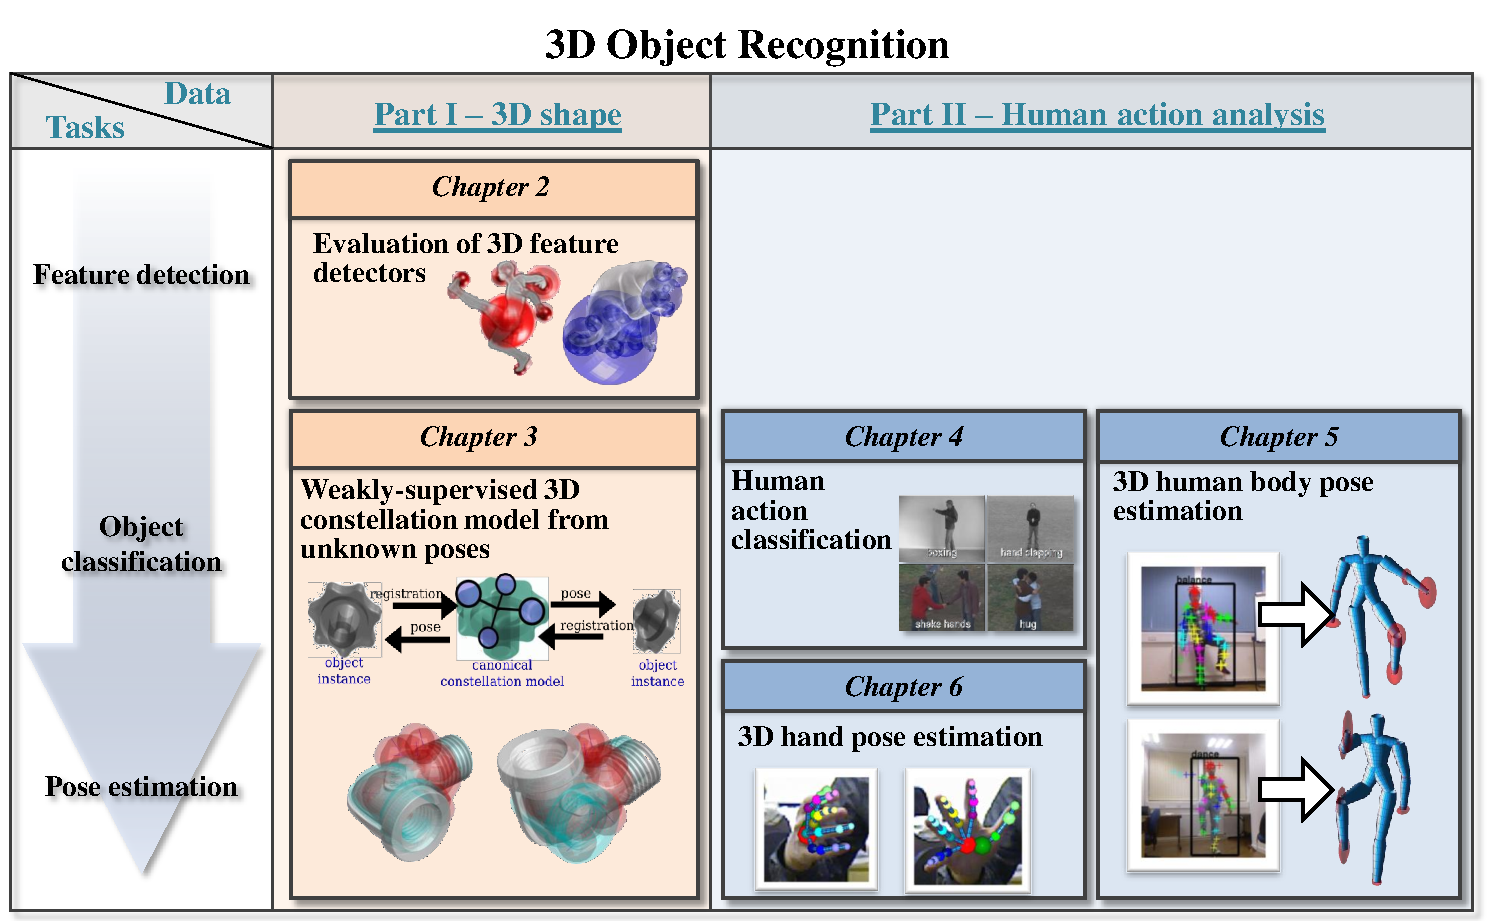
\includegraphics[width=1\linewidth]{./fig/intro/intro.pdf}
\caption{\textbf{Thesis outline}} 
\label{fig/intro/outline}
\end{figure}

\section{Thesis overview}

\subsection{Contributions}

The main contributions of this thesis are:
\begin{itemize}
	\item A detailed performance evaluation on several state-of-the-art 3D interest point detectors.
	\item A new weakly-supervised constellation model for simultaneous 3D shape recognition and registration, using training data with unknown pose. 
	\item A real-time algorithm that combines appearance and structural information for video-based action classification using semantic texton forest. 
	\item A new technique to estimate 3D human body poses using action detection and regression random forests. 
	\item A semi-supervised 3D hand pose estimation system that combines synthetic and realistic training data. 
\end{itemize}

\subsection{Limiting the scope}

% Some thing which is not considered?
In order to concentrate on the most important and relevant topics, 
several applications are not considered within this thesis. 
The first is recognition of 3D meshes \cite{Zaharescu2009, Bronstein2011, Kokkinos2012}. Textured mesh is a standard representation of 3D shapes in computer graphics and computer-aided design (CAD) tasks. However, realistic 3D shape data are usually captured in textureless point clouds, depthmaps or voxels. In addition, instances of the same object class can have very different textures, texture-based features are therefore not suitable for shape classification.      

The second application is model-based 3D object recognition, \eg \cite{Mian2006, Rothganger2006, Shang2010}. A pose estimator is trained on different objects in a specific scene, rather than object instances from the same class. The performances of object recognition and pose estimation of such approach rely mainly on feature matching between the model and query object instance. 

Thirdly, marker-based motion capture sysems are not included in the scope of this thesis. They have been widely employed in computer-generated imagery for films and games. Markers are localised accurately from a calibrated camera system, using simple computer vision techniques. Poses are estimated straightforwardly by mapping the markers to a predefined articulated skeleton.
 With a calibrated camera network, 3D human poses can be recovered using marker-based approaches easily.  

Finally, body shape estimation from images and videos are not considered in the thesis \cite{Guan2009, Rother2009, Chen2011}. It reconstructs 3D human shapes directly from testing data, instead of parameterised poses of a articulated model. Body pose estimation is concerned with understanding the semantics of the subject and the scene, rather than reconstructing them accurately. 

\subsection{Outline}

This thesis is outlined in figure \ref{fig/intro/outline}. In the first part, chapter \ref{chap/eval} and chapter \ref{chap/reg} focus on the recognition and pose estimation of 3D shapes; the second part, chapter \ref{chap/act} -- \ref{chap/hand}, focuses on human action analysis, including action categorisation and 3D pose estimation of human body and hand gestures. Chapter \ref{chap/conclusion} concludes the thesis with possible directions for future research. 

\subsection*{Part I --- 3D Shape}

%\paragraph{Chapter 2.} This chapter presents a literature review of 3D shape processing techniques.  Recent topics about 3D feature detection, shape representation, shape recognition and pose estimation are discussed.  

\subsubsection*{Chapter 2. Evaluation of 3D feature detectors} 
A performance evaluation of volumetric 3D interest points is presented in this chapter. 
It first gives a brief introduction to the volumetric interest point detectors used in existing literature.
There interest point detectors are evaluated quantitatively using a new performance metric.
Finally, qualitative characteristics of the candidate detectors are also discussed in this chapter. 

\subsubsection*{Chapter 3. 3D Constellation model from unkown pose}
This chapter presents a weakly supervised constellation model for simultaneous 3D shape recognition and pose estimation. 
The proposed model learns the shape, appearance and pose of an object class from training exemplars, \eg images or point clouds, which contain examples of the object in unknown poses.  

\subsection*{Part II --- Human action analysis}

%\paragraph{Chapter 5.} This chapter introduces various sub-problems in human action analysis, including human action recognition, body pose estimation and hand pose estimation.  It discusses the application of random forests and its variants to model human actions and poses. It also reviews the existing approaches for the above sub-problems. 

\subsubsection*{Chapter 4. Human action classification} 
This chapter addresses the recognition sub-problem in human action analysis. A spatiotemporal semantic and structural forest is proposed to recognise human actions in real-time.    

\subsubsection*{Chapter 5. 3D human body pose estimation} 
This chapter presents a new approach to 3D body pose estimation in unconstrained, monoculat videos. 
A new hybrid decision forest is introduced, in order to perform action detection and pose estimation simultaneously. 
Pose estimation is based on action detection, which includes joint classification and localisation of actions in videos. 
% By combining regression random forests with action detection, the proposed method infers 3D poses from unconstrained, monocular videos. 

\subsubsection*{Chapter 6. 3D hand pose estimation} 
This chapter addresses the sub-problem of 3D hand pose estimation. 
The regression tree learning algorithm introduced in chapter \ref{chap/body} is further developed to estimate 3D hand pose from different viewpoints. 
A data-driven inverse kinematic scheme is also described to refine the occluded joints.
